\documentclass[11pt,a4paper]{article}

\usepackage[utf8]{inputenc}
\usepackage[T1]{fontenc}
\usepackage[brazil]{babel}
\usepackage{amsmath}
\usepackage{amssymb}
\usepackage{booktabs}
\usepackage{longtable}
\usepackage{array}
\usepackage{graphicx}
\usepackage{xcolor}
\usepackage{tikz}
\usetikzlibrary{shapes.geometric,arrows.meta,positioning,decorations.pathreplacing,calc}
\usepackage[hidelinks]{hyperref}

\tikzset{
  bloco/.style={rectangle,rounded corners=2pt,draw=black!55,fill=black!4,align=center,minimum height=6mm,inner sep=2mm,font=\small},
  blocoI/.style={bloco,fill=blue!6},
  blocoG/.style={bloco,fill=teal!8},
  seta/.style={-{Latex[length=2.1mm]},semithick,black!65},
  rotulo/.style={font=\scriptsize,black!55,align=left},
}

\newcommand{\code}[1]{\texttt{#1}}

\title{Comparação entre ILS e GRASP na otimização do Índice de Qualidade Caminhável (IQC):\\ análise estatística dos resultados}
\author{}
\date{}

\begin{document}

\maketitle

\section{Escopo e fontes de dados}
\label{sec:comp-escopo}

Este capítulo compara os dois métodos implementados no projeto, o Iterated Local Search (ILS) e o GRASP, exclusivamente a partir dos resultados que eles produziram sobre as mesmas instâncias. Todos os números vêm dos arquivos gravados em \code{results/ils/} e \code{results/grasp/} e dos conjuntos de dados de caminhabilidade em \code{data/location/}; nenhuma informação externa a esses arquivos é usada.

A configuração do ILS usada na comparação é a de força de perturbação $2$, que foi a melhor das duas configurações testadas para o método nas quinze instâncias, conforme a análise do capítulo do ILS. A comparação com a configuração de força $10$ é reportada de forma resumida onde couber. O GRASP é comparado na sua única configuração, com $\alpha$ sorteado uniformemente em $[0,1]$ a cada iteração.

\section{Os métodos comparados}
\label{sec:comp-metodos}

Os dois métodos resolvem exatamente o mesmo problema: alocar $100$ POIs em pares (hexágono de origem, dimensão) para maximizar a soma do IQC, avaliada pela mesma função objetivo, sobre o mesmo espaço de soluções. Eles compartilham o operador de busca local, por primeira melhora com movimento de realocação que preserva a dimensão, com os mesmos parâmetros ($64$ vizinhos por passo, $25$ passos). A diferença entre eles está em como cada um gera os pontos de partida da busca local e em como conecta as iterações, e a Figura~\ref{fig:comp-arq} resume essa diferença.

O ILS mantém uma única cadeia: parte de uma alocação aleatória, desce a um ótimo local e, a cada iteração, perturba o ótimo local corrente, reotimiza e decide pela aceitação (\code{Better}); a perturbação tem força adaptativa. O GRASP não mantém estado entre iterações: a cada iteração constrói uma solução nova do zero, por construção gulosa randomizada com escore surrogate e RCL, aplica a busca local e guarda apenas a melhor solução já vista. Em resumo, o ILS explora a vizinhança de uma boa solução ao longo do tempo, e o GRASP amostra repetidamente construções independentes.

\begin{figure}[htbp]
\centering
\begin{tikzpicture}[node distance=3.2mm and 4mm]
% coluna ILS
\node[blocoI] (i0) {alocação aleatória $s_0$};
\node[blocoI,below=of i0] (i1) {busca local $\rightarrow s^\ast$};
\node[blocoI,below=of i1] (i2) {perturbação de $s^\ast$};
\node[blocoI,below=of i2] (i3) {busca local};
\node[blocoI,below=of i3] (i4) {aceitação \code{Better}};
\draw[seta] (i0) -- (i1);
\draw[seta] (i1) -- (i2);
\draw[seta] (i2) -- (i3);
\draw[seta] (i3) -- (i4);
\draw[seta] (i4.west) -- ++(-7mm,0) |- (i2.west);
\node[rotulo,above=1.5mm of i0] {\textbf{ILS}: uma única cadeia};
% coluna GRASP
\node[blocoG,right=38mm of i0] (g0) {sorteia $\alpha$};
\node[blocoG,below=of g0] (g1) {construção randomizada (RCL)};
\node[blocoG,below=of g1] (g2) {busca local};
\node[blocoG,below=of g2] (g3) {atualiza melhor solução};
\draw[seta] (g0) -- (g1);
\draw[seta] (g1) -- (g2);
\draw[seta] (g2) -- (g3);
\draw[seta] (g3.west) -- ++(-5mm,0) |- (g0.west);
\node[rotulo,above=1.5mm of g0] {\textbf{GRASP}: reinícios independentes};
\end{tikzpicture}
\caption{Arquitetura das iterações dos dois métodos, como implementados. Os blocos de busca local são o mesmo operador nos dois casos; a diferença está na origem do ponto de partida de cada iteração (perturbação do ótimo corrente no ILS; construção nova no GRASP) e na memória entre iterações (a cadeia do ILS contra o reinício do GRASP).}
\label{fig:comp-arq}
\end{figure}

A Tabela~\ref{tab:comp-config} resume as configurações. Os elementos compartilhados garantem que a comparação isola a diferença de estratégia: mesmo problema, mesma função objetivo, mesma busca local, mesmas $100$ sementes, mesmo teto de $30\,000$ avaliações e mesmos limites de $500$ iterações e $80$ iterações sem melhora.

\begin{table}[htbp]
\centering
\caption{Configuração dos dois métodos na comparação.}
\label{tab:comp-config}
\renewcommand{\arraystretch}{1.2}
\begin{tabular}{@{}lll@{}}
\toprule
Elemento & ILS (força $2$) & GRASP \\
\midrule
Solução inicial da iteração & perturbação do ótimo corrente & construção randomizada (RCL) \\
Memória entre iterações & cadeia única, aceitação \code{Better} & nenhuma (guarda só a melhor) \\
Parâmetro específico & força $2$, bloco $2$, adaptativa & $\alpha \sim U[0,1]$ por iteração \\
Busca local & \multicolumn{2}{c}{idêntica: primeira melhora, $64$ vizinhos, $25$ passos} \\
Avaliações (teto) & \multicolumn{2}{c}{$30\,000$ por semente} \\
Outros limites & \multicolumn{2}{c}{$500$ iterações; $80$ iterações sem melhora} \\
Sementes & \multicolumn{2}{c}{as mesmas $100$ de \code{seeds.txt}} \\
Instâncias & \multicolumn{2}{c}{$5$ localidades $\times$ $3$ perfis $= 15$} \\
\bottomrule
\end{tabular}
\end{table}

\section{Desenho experimental e metodologia estatística}
\label{sec:comp-metodologia}

Cada método executou uma vez por semente em cada instância, com as mesmas $100$ sementes, o que dá $1\,500$ execuções por método. Como as sementes coincidem, a comparação principal é pareada: para cada instância, comparam-se, semente a semente, os melhores valores finais dos dois métodos. Vale registrar o que o pareamento significa aqui: a semente alimenta os dois métodos, mas governa mecanismos diferentes em cada um (alocação inicial e movimentos no ILS; sorteios da RCL e da busca local no GRASP), de modo que o pareamento funciona como bloqueio pela semente, e sua utilidade efetiva é medida adiante pela correlação entre os pares.

Os instrumentos são os mesmos dos capítulos anteriores. Por instância: diferença média pareada com intervalo de confiança de $95\%$ ($\bar{d} \pm t_{0{,}975;\,99}\, s_d/\sqrt{100}$), teste de postos sinalizados de Wilcoxon com correção de Holm para os quinze testes, contagem de vitórias por semente e correlação bisserial de postos pareada $r_{rb}$ como tamanho de efeito ($r_{rb} = (W^+ - W^-)/(W^+ + W^-)$, em que $W^+$ e $W^-$ são as somas de postos das diferenças positivas e negativas; $r_{rb} = \pm 1$ indica dominância completa). No nível agregado, a unidade de análise passa a ser a instância: aplica-se o teste de Wilcoxon às quinze diferenças médias e o teste do sinal à contagem de instâncias vencidas, porque as $1\,500$ diferenças por semente não são independentes entre si dentro de uma mesma instância. A igualdade de variâncias entre métodos é testada por Brown--Forsythe (teste de Levene centrado na mediana), também com Holm. A comparação sob orçamento igual usa o melhor valor acumulado em marcos de avaliações, extraído das trajetórias, pareado por semente. A análise de avaliações até o alvo fixa, por instância, o alvo como a média final do método mais fraco naquela instância, e mede, por semente, o número de avaliações que cada método levou para alcançá-lo, reportando a fração de sementes que o alcançou e a mediana entre as que alcançaram.

Duas ressalvas de medição. Primeiro, o tempo de execução dos dois métodos foi medido em sessões diferentes; a medida de esforço robusta e independente de máquina é o número de avaliações da função objetivo, que é idêntica nos dois métodos, e é ela que fundamenta as comparações de custo. Segundo, o GRASP para por estagnação antes de esgotar o orçamento, então a comparação dos valores finais favorece o método que usa mais orçamento; a Seção~\ref{sec:comp-orcamento} elimina essa assimetria comparando os métodos nos mesmos marcos de avaliações.

\section{Qualidade final por instância}
\label{sec:comp-final}

A Tabela~\ref{tab:comp-final} apresenta a comparação pareada dos valores finais, e as Figuras~\ref{fig:comp-box} e~\ref{fig:comp-forest} a resumem graficamente. O GRASP obteve média maior em onze das quinze instâncias; o ILS, em quatro (as três de Itajubá e Milão/atleta). Todas as quinze diferenças são estatisticamente significativas após a correção de Holm ($p_{\text{Holm}} \le 1{,}1 \times 10^{-9}$ em todas), e os tamanhos de efeito são grandes: $|r_{rb}| \ge 0{,}70$ em todas as instâncias, com dominância completa por semente ($100 \times 0$) em nove delas.

\renewcommand{\arraystretch}{1.15}
\begin{longtable}{@{}l l c c r c c r@{}}
\caption{Comparação pareada dos valores finais (soma de IQC; $100$ sementes por instância). Diferença $= $ GRASP $-$ ILS, com IC de $95\%$; vitórias contam sementes; $r_{rb}$ é a correlação bisserial de postos. Todas as diferenças são significativas após Holm ($p_{\text{Holm}} \le 1{,}1\times10^{-9}$).}\label{tab:comp-final}\\
\toprule
Localidade & Perfil & ILS média (dp) & GRASP média (dp) & Dif. & IC $95\%$ & Vit.\ G$\times$I & $r_{rb}$ \\
\midrule
\endfirsthead
\toprule
Localidade & Perfil & ILS média (dp) & GRASP média (dp) & Dif. & IC $95\%$ & Vit.\ G$\times$I & $r_{rb}$ \\
\midrule
\endhead
av\_paulista & athlete & 59,04 (0,44) & 60,21 (0,37) & $+1{,}168$ & $[+1{,}05;\ +1{,}29]$ & 98$\times$2 & $+0{,}998$ \\
av\_paulista & average\_adult & 51,08 (0,31) & 53,43 (0,46) & $+2{,}352$ & $[+2{,}25;\ +2{,}46]$ & 100$\times$0 & $+1{,}000$ \\
av\_paulista & elderly & 42,12 (0,21) & 44,87 (0,42) & $+2{,}748$ & $[+2{,}66;\ +2{,}83]$ & 100$\times$0 & $+1{,}000$ \\
itajuba\_centro & athlete & 49,60 (1,31) & 43,27 (0,71) & $-6{,}333$ & $[-6{,}65;\ -6{,}02]$ & 0$\times$100 & $-1{,}000$ \\
itajuba\_centro & average\_adult & 43,55 (1,58) & 38,40 (0,81) & $-5{,}143$ & $[-5{,}49;\ -4{,}79]$ & 0$\times$100 & $-1{,}000$ \\
itajuba\_centro & elderly & 35,67 (1,38) & 32,99 (0,69) & $-2{,}675$ & $[-3{,}00;\ -2{,}35]$ & 5$\times$95 & $-0{,}981$ \\
metro\_ana\_rosa & athlete & 50,22 (0,76) & 53,15 (0,60) & $+2{,}925$ & $[+2{,}73;\ +3{,}12]$ & 100$\times$0 & $+1{,}000$ \\
metro\_ana\_rosa & average\_adult & 44,65 (0,44) & 47,77 (0,57) & $+3{,}121$ & $[+2{,}98;\ +3{,}27]$ & 100$\times$0 & $+1{,}000$ \\
metro\_ana\_rosa & elderly & 36,56 (0,26) & 37,06 (0,38) & $+0{,}507$ & $[+0{,}41;\ +0{,}61]$ & 83$\times$17 & $+0{,}855$ \\
milao\_italia & athlete & 65,30 (0,22) & 64,99 (0,13) & $-0{,}306$ & $[-0{,}36;\ -0{,}26]$ & 18$\times$82 & $-0{,}901$ \\
milao\_italia & average\_adult & 59,62 (0,20) & 59,90 (0,27) & $+0{,}280$ & $[+0{,}21;\ +0{,}35]$ & 79$\times$21 & $+0{,}733$ \\
milao\_italia & elderly & 51,34 (0,15) & 52,60 (0,14) & $+1{,}256$ & $[+1{,}22;\ +1{,}30]$ & 100$\times$0 & $+1{,}000$ \\
shinjuku\_toquio & athlete & 60,03 (0,31) & 60,25 (0,19) & $+0{,}224$ & $[+0{,}16;\ +0{,}28]$ & 78$\times$22 & $+0{,}703$ \\
shinjuku\_toquio & average\_adult & 53,95 (0,29) & 55,10 (0,31) & $+1{,}158$ & $[+1{,}08;\ +1{,}24]$ & 100$\times$0 & $+1{,}000$ \\
shinjuku\_toquio & elderly & 44,39 (0,26) & 46,74 (0,36) & $+2{,}350$ & $[+2{,}27;\ +2{,}43]$ & 100$\times$0 & $+1{,}000$ \\
\bottomrule
\end{longtable}

\begin{figure}[htbp]
\centering
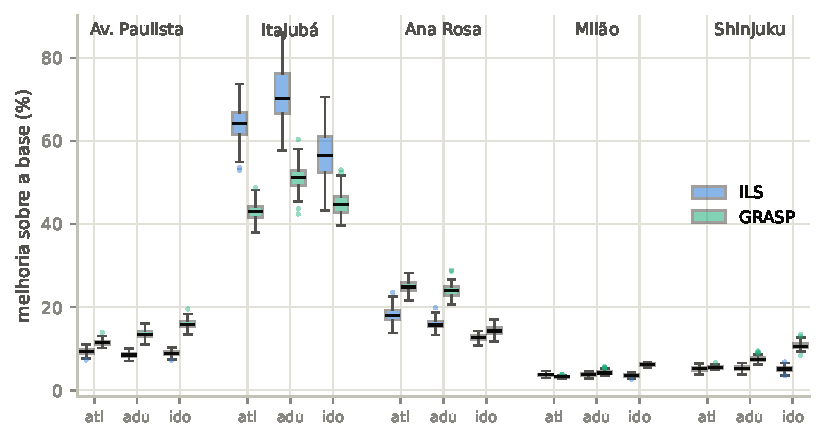
\includegraphics[width=\textwidth]{figures/comp_box.pdf}
\caption{Distribuição, entre as $100$ sementes, da melhoria porcentual sobre a linha de base, por instância e método.}
\label{fig:comp-box}
\end{figure}

\begin{figure}[htbp]
\centering
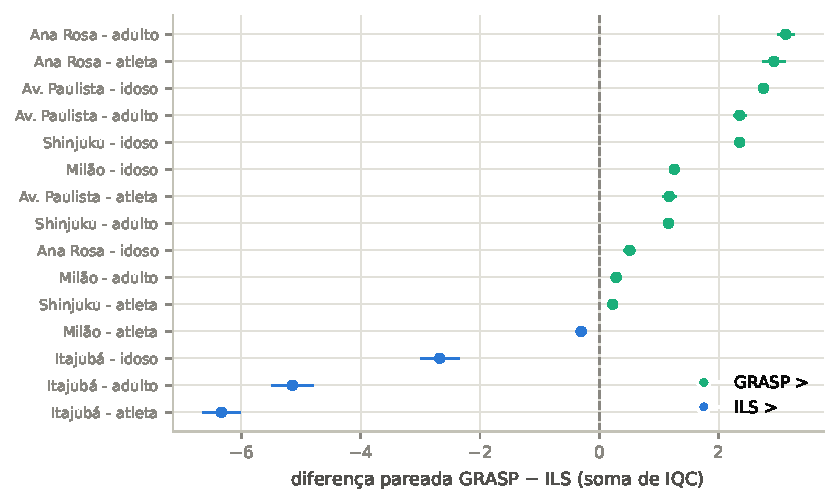
\includegraphics[width=0.8\textwidth]{figures/comp_forest.pdf}
\caption{Diferença média pareada (GRASP $-$ ILS) por instância, com intervalos de confiança de $95\%$, ordenada pelo valor da diferença. Os intervalos não cruzam o zero em nenhuma instância.}
\label{fig:comp-forest}
\end{figure}

No nível agregado, com a instância como unidade de análise, a vantagem numérica do GRASP (onze instâncias em quinze) não atinge significância: o teste do sinal dá $p = 0{,}118$ e o teste de Wilcoxon sobre as quinze diferenças médias dá $p = 0{,}330$. A razão é visível na Figura~\ref{fig:comp-forest}: as três diferenças de Itajubá, a favor do ILS, são muito maiores em módulo (de $2{,}7$ a $6{,}3$) do que a maioria das diferenças a favor do GRASP (de $0{,}2$ a $3{,}1$). Os dados portanto não sustentam a afirmação de que um método é superior ao outro em geral; sustentam que o resultado depende fortemente da instância, com o GRASP à frente na maior parte delas e o ILS à frente, por margens grandes, no grupo de Itajubá. Contra a configuração de força $10$ do ILS, o GRASP obteve média maior em doze das quinze instâncias.

O mesmo padrão se repete quando se olha apenas para a melhor solução global de cada método (o máximo sobre as $100$ sementes): o GRASP tem o melhor valor em onze instâncias e o ILS nas mesmas quatro (Tabela~\ref{tab:comp-best}).

\begin{table}[htbp]
\centering
\caption{Melhor solução global (máximo sobre as $100$ sementes) por instância e método.}
\label{tab:comp-best}
\renewcommand{\arraystretch}{1.12}
\begin{tabular}{@{}l l c c@{}}
\toprule
Localidade & Perfil & ILS & GRASP \\
\midrule
av\_paulista & athlete & 59,98 & \textbf{61,50} \\
av\_paulista & average\_adult & 51,75 & \textbf{54,60} \\
av\_paulista & elderly & 42,68 & \textbf{46,24} \\
itajuba\_centro & athlete & \textbf{52,53} & 44,97 \\
itajuba\_centro & average\_adult & \textbf{47,30} & 40,76 \\
itajuba\_centro & elderly & \textbf{38,81} & 34,82 \\
metro\_ana\_rosa & athlete & 52,55 & \textbf{54,56} \\
metro\_ana\_rosa & average\_adult & 46,18 & \textbf{49,65} \\
metro\_ana\_rosa & elderly & 37,08 & \textbf{37,96} \\
milao\_italia & athlete & \textbf{65,84} & 65,34 \\
milao\_italia & average\_adult & 60,04 & \textbf{60,68} \\
milao\_italia & elderly & 51,68 & \textbf{52,88} \\
shinjuku\_toquio & athlete & 60,77 & \textbf{60,89} \\
shinjuku\_toquio & average\_adult & 54,63 & \textbf{56,14} \\
shinjuku\_toquio & elderly & 45,11 & \textbf{47,92} \\
\bottomrule
\end{tabular}
\end{table}

A Figura~\ref{fig:comp-scatter} mostra os pares semente a semente em duas instâncias, uma vencida por cada método: as nuvens ficam inteiramente de um lado da reta identidade, o que ilustra a dominância medida pelos $r_{rb}$ próximos de $\pm 1$. A Figura~\ref{fig:comp-ecdf} apresenta as funções de distribuição acumulada empíricas dos valores finais nas duas instâncias representativas usadas ao longo dos capítulos: em Itajubá as curvas não se cruzam a favor do ILS; em Milão/idoso, a favor do GRASP.

\begin{figure}[htbp]
\centering
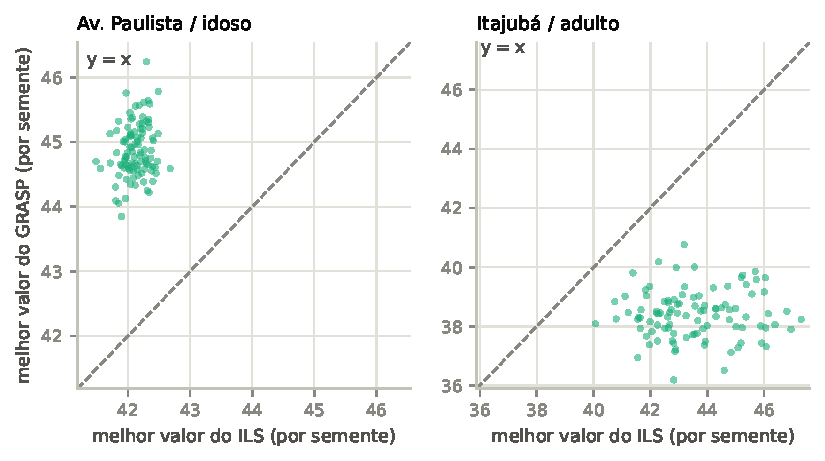
\includegraphics[width=\textwidth]{figures/comp_scatter.pdf}
\caption{Melhor valor do GRASP contra o melhor valor do ILS, semente a semente. À esquerda, instância vencida pelo GRASP; à direita, vencida pelo ILS. A reta tracejada é a identidade.}
\label{fig:comp-scatter}
\end{figure}

\begin{figure}[htbp]
\centering
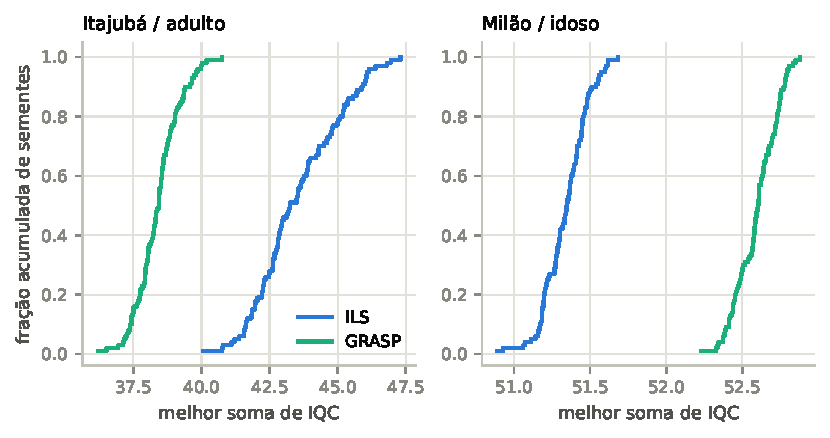
\includegraphics[width=\textwidth]{figures/comp_ecdf.pdf}
\caption{Distribuição acumulada empírica dos valores finais das $100$ sementes, por método, nas duas instâncias representativas.}
\label{fig:comp-ecdf}
\end{figure}

Um detalhe metodológico medido nos dados: a correlação de Spearman entre os pares (valor do GRASP, valor do ILS na mesma semente) é fraca e de sinal variável entre instâncias (de $-0{,}22$ a $+0{,}29$; três instâncias com $p$ nominal abaixo de $0{,}05$, nenhuma sobrevivendo à correção de Holm). Ou seja, uma semente boa para um método não tende a ser boa para o outro — coerente com o fato de a semente alimentar mecanismos diferentes em cada método. O pareamento permanece válido como bloqueio, mas na prática as amostras se comportam como independentes.

\subsection{Dispersão entre sementes}

A Tabela~\ref{tab:comp-var} compara os desvios padrão. O teste de Brown--Forsythe rejeita a igualdade de variâncias, após Holm, em oito das quinze instâncias, sem direção uniforme: o GRASP é menos disperso nas três instâncias de Itajubá (desvios de $0{,}69$ a $0{,}81$ contra $1{,}31$ a $1{,}58$ do ILS) e nos perfis atleta de Milão e Shinjuku; o ILS é menos disperso em av\_paulista (adulto e idoso) e em Ana Rosa/idoso. Não há, portanto, um método uniformemente mais estável entre sementes; a dispersão relativa também depende da instância.

\begin{table}[htbp]
\centering
\caption{Desvios padrão dos valores finais e teste de igualdade de variâncias de Brown--Forsythe (BF). O símbolo $^{\dagger}$ marca $p_{\text{Holm}} < 0{,}05$.}
\label{tab:comp-var}
\renewcommand{\arraystretch}{1.12}
\begin{tabular}{@{}l l c c c@{}}
\toprule
Localidade & Perfil & dp ILS & dp GRASP & $p$ BF (Holm) \\
\midrule
av\_paulista & athlete & 0,436 & 0,374 & 0,354 \\
av\_paulista & average\_adult & 0,307 & 0,461 & 0,001$^{\dagger}$ \\
av\_paulista & elderly & 0,211 & 0,419 & $<0{,}001^{\dagger}$ \\
itajuba\_centro & athlete & 1,313 & 0,710 & $<0{,}001^{\dagger}$ \\
itajuba\_centro & average\_adult & 1,578 & 0,811 & $<0{,}001^{\dagger}$ \\
itajuba\_centro & elderly & 1,376 & 0,691 & $<0{,}001^{\dagger}$ \\
metro\_ana\_rosa & athlete & 0,761 & 0,604 & 0,165 \\
metro\_ana\_rosa & average\_adult & 0,444 & 0,573 & 0,091 \\
metro\_ana\_rosa & elderly & 0,261 & 0,378 & 0,012$^{\dagger}$ \\
milao\_italia & athlete & 0,218 & 0,126 & $<0{,}001^{\dagger}$ \\
milao\_italia & average\_adult & 0,201 & 0,267 & 0,354 \\
milao\_italia & elderly & 0,146 & 0,138 & 1,000 \\
shinjuku\_toquio & athlete & 0,308 & 0,189 & $<0{,}001^{\dagger}$ \\
shinjuku\_toquio & average\_adult & 0,290 & 0,305 & 1,000 \\
shinjuku\_toquio & elderly & 0,262 & 0,357 & 0,165 \\
\bottomrule
\end{tabular}
\end{table}

\section{Comparação sob orçamento igual de avaliações}
\label{sec:comp-orcamento}

Como o GRASP parou por estagnação em todas as execuções, usando em média $9\,561$ avaliações, e o ILS usou praticamente o teto ($30\,101$ em média, contando o excedente da última busca local), a comparação dos valores finais mistura qualidade com quantidade de orçamento consumido. Esta seção remove essa assimetria comparando o melhor valor acumulado dos dois métodos nos mesmos marcos de avaliações, pareado por semente.

A Tabela~\ref{tab:comp-cp} mostra a diferença média pareada em quatro marcos. Três fatos se destacam. Primeiro, em $1\,000$ avaliações o GRASP está à frente em doze das quinze instâncias; de $5\,000$ em diante o quadro se estabiliza em onze a quatro, o mesmo do resultado final — ou seja, o placar por instância não é artefato da diferença de orçamento consumido. Segundo, nas instâncias de Itajubá a vantagem do ILS cresce com o orçamento (por exemplo, de $-2{,}83$ em $1\,000$ avaliações para $-6{,}33$ em $30\,000$ no perfil atleta): o ILS continua convertendo orçamento em melhora, enquanto o GRASP satura. Terceiro, Milão/atleta é a única instância em que o sinal muda ao longo do orçamento: o GRASP está à frente em $1\,000$ avaliações ($+0{,}07$) e o ILS o ultrapassa a partir de $5\,000$ ($-0{,}11$, chegando a $-0{,}31$ no final).

\renewcommand{\arraystretch}{1.12}
\begin{longtable}{@{}l l r r r r@{}}
\caption{Diferença média pareada (GRASP $-$ ILS) do melhor valor acumulado em marcos de avaliações.}\label{tab:comp-cp}\\
\toprule
Localidade & Perfil & $1\,000$ & $5\,000$ & $10\,000$ & $30\,000$ \\
\midrule
\endfirsthead
\toprule
Localidade & Perfil & $1\,000$ & $5\,000$ & $10\,000$ & $30\,000$ \\
\midrule
\endhead
av\_paulista & athlete & $+1{,}60$ & $+1{,}35$ & $+1{,}28$ & $+1{,}17$ \\
av\_paulista & average\_adult & $+2{,}18$ & $+2{,}43$ & $+2{,}44$ & $+2{,}35$ \\
av\_paulista & elderly & $+2{,}53$ & $+2{,}76$ & $+2{,}79$ & $+2{,}75$ \\
itajuba\_centro & athlete & $-2{,}83$ & $-4{,}55$ & $-5{,}33$ & $-6{,}33$ \\
itajuba\_centro & average\_adult & $-1{,}78$ & $-3{,}40$ & $-4{,}01$ & $-5{,}14$ \\
itajuba\_centro & elderly & $-0{,}75$ & $-1{,}97$ & $-2{,}21$ & $-2{,}67$ \\
metro\_ana\_rosa & athlete & $+2{,}97$ & $+2{,}92$ & $+3{,}08$ & $+2{,}93$ \\
metro\_ana\_rosa & average\_adult & $+2{,}74$ & $+3{,}06$ & $+3{,}15$ & $+3{,}12$ \\
metro\_ana\_rosa & elderly & $+0{,}57$ & $+0{,}55$ & $+0{,}59$ & $+0{,}51$ \\
milao\_italia & athlete & $+0{,}07$ & $-0{,}11$ & $-0{,}19$ & $-0{,}31$ \\
milao\_italia & average\_adult & $+0{,}48$ & $+0{,}38$ & $+0{,}38$ & $+0{,}28$ \\
milao\_italia & elderly & $+1{,}28$ & $+1{,}32$ & $+1{,}33$ & $+1{,}26$ \\
shinjuku\_toquio & athlete & $+0{,}43$ & $+0{,}34$ & $+0{,}32$ & $+0{,}23$ \\
shinjuku\_toquio & average\_adult & $+1{,}12$ & $+1{,}19$ & $+1{,}23$ & $+1{,}16$ \\
shinjuku\_toquio & elderly & $+1{,}99$ & $+2{,}32$ & $+2{,}42$ & $+2{,}35$ \\
\bottomrule
\end{longtable}

A Figura~\ref{fig:comp-conv} sobrepõe as curvas de convergência médias dos dois métodos nas duas instâncias representativas. Em Itajubá/adulto, o GRASP parte na frente nas primeiras centenas de avaliações e é ultrapassado pelo ILS por volta de algumas centenas de avaliações, com a distância crescendo até o final. Em Milão/idoso, o GRASP domina do início ao fim, com a curva do ILS saturando em um patamar mais baixo.

\begin{figure}[htbp]
\centering
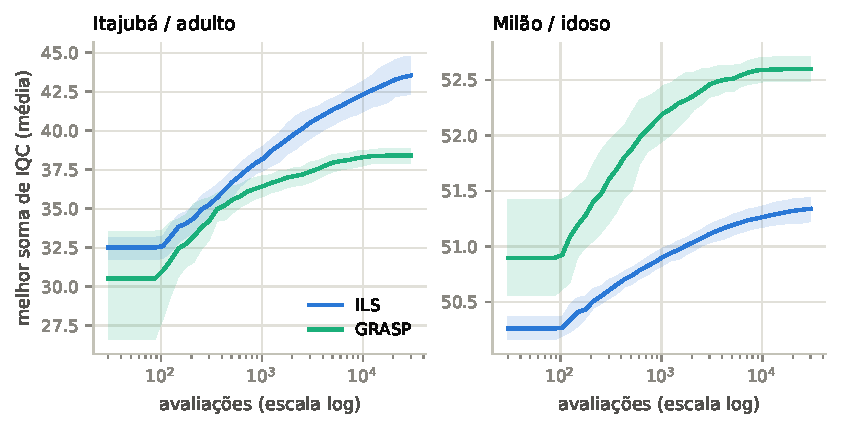
\includegraphics[width=\textwidth]{figures/comp_convergence.pdf}
\caption{Convergência média (linhas) e faixas interquartílicas (áreas), por método, nas duas instâncias representativas, em escala logarítmica de avaliações.}
\label{fig:comp-conv}
\end{figure}

\subsection{Avaliações até o alvo}

A Tabela~\ref{tab:comp-ttt} fixa, por instância, o alvo como a média final do método mais fraco, e mede quanto orçamento cada método levou para alcançá-lo. Por construção, o método mais fraco alcança o próprio alvo em cerca de metade das sementes; o interessante é a velocidade do método mais forte. Nas onze instâncias vencidas pelo GRASP, ele alcança a média final do ILS com medianas entre $148$ e $2\,990$ avaliações — em oito delas com menos de $600$ avaliações, ou seja, com menos de $2\%$ do orçamento que o ILS consumiu para chegar ao mesmo nível. Nas três instâncias de Itajubá, o quadro se inverte: o ILS alcança a média final do GRASP com medianas entre $648$ e $1\,461$ avaliações, enquanto o GRASP só alcança o próprio nível final na metade das sementes. A Figura~\ref{fig:comp-ttt} mostra as distribuições acumuladas nas duas instâncias representativas, uma imagem espelhada da outra.

\renewcommand{\arraystretch}{1.12}
\begin{longtable}{@{}l l c c c c c@{}}
\caption{Avaliações até o alvo (alvo $=$ média final do método mais fraco na instância). ``Alc.'' é a fração de sementes que alcançou o alvo; a mediana é calculada entre as que alcançaram.}\label{tab:comp-ttt}\\
\toprule
Localidade & Perfil & Alvo & Alc.\ ILS & Med.\ ILS & Alc.\ GRASP & Med.\ GRASP \\
\midrule
\endfirsthead
\toprule
Localidade & Perfil & Alvo & Alc.\ ILS & Med.\ ILS & Alc.\ GRASP & Med.\ GRASP \\
\midrule
\endhead
av\_paulista & athlete & 59,04 & 0,51 & 6\,792 & 1,00 & 511 \\
av\_paulista & average\_adult & 51,08 & 0,47 & 5\,632 & 1,00 & 176 \\
av\_paulista & elderly & 42,12 & 0,48 & 6\,566 & 1,00 & 148 \\
itajuba\_centro & athlete & 43,27 & 1,00 & 648 & 0,50 & 2\,899 \\
itajuba\_centro & average\_adult & 38,40 & 1,00 & 1\,187 & 0,51 & 4\,734 \\
itajuba\_centro & elderly & 32,99 & 0,97 & 1\,461 & 0,44 & 4\,022 \\
metro\_ana\_rosa & athlete & 50,22 & 0,50 & 5\,901 & 1,00 & 336 \\
metro\_ana\_rosa & average\_adult & 44,65 & 0,44 & 4\,373 & 1,00 & 249 \\
metro\_ana\_rosa & elderly & 36,56 & 0,45 & 6\,265 & 0,90 & 1\,896 \\
milao\_italia & athlete & 64,99 & 0,90 & 3\,065 & 0,51 & 2\,990 \\
milao\_italia & average\_adult & 59,62 & 0,52 & 10\,051 & 0,92 & 1\,866 \\
milao\_italia & elderly & 51,34 & 0,53 & 7\,932 & 1,00 & 217 \\
shinjuku\_toquio & athlete & 60,03 & 0,52 & 5\,273 & 0,91 & 1\,882 \\
shinjuku\_toquio & average\_adult & 53,95 & 0,50 & 4\,075 & 1,00 & 270 \\
shinjuku\_toquio & elderly & 44,39 & 0,48 & 4\,949 & 1,00 & 162 \\
\bottomrule
\end{longtable}

\begin{figure}[htbp]
\centering
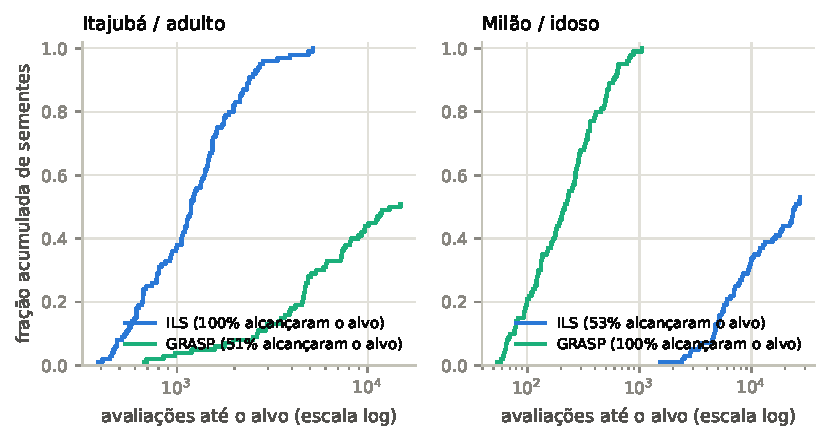
\includegraphics[width=\textwidth]{figures/comp_ttt.pdf}
\caption{Distribuição acumulada do número de avaliações necessárias para alcançar o alvo, por método, nas duas instâncias representativas. As legendas indicam a fração de sementes que alcançou o alvo dentro da execução.}
\label{fig:comp-ttt}
\end{figure}

\section{Custo computacional e critérios de parada}
\label{sec:comp-custo}

A Tabela~\ref{tab:comp-custo} compara o consumo de recursos. Os motivos de parada são opostos: o ILS esgotou o orçamento de avaliações em $1\,461$ das $1\,500$ execuções (as demais $39$ pararam por estagnação), enquanto o GRASP parou por estagnação em todas as $1\,500$, consumindo em média $9\,561$ avaliações, cerca de $32\%$ do teto — a Figura~\ref{fig:comp-orc} visualiza essa diferença. O tempo médio por semente foi de $71{,}1$ segundos para o ILS e $21{,}4$ para o GRASP, uma razão de $3{,}3$, próxima da razão de avaliações ($3{,}1$), o que é esperado dado que a avaliação domina o tempo nos dois métodos; vale a ressalva de que os tempos foram medidos em sessões distintas, e a medida robusta é o número de avaliações.

\renewcommand{\arraystretch}{1.12}
\begin{longtable}{@{}l l r r r r@{}}
\caption{Custo médio por semente: avaliações da função objetivo e tempo (s).}\label{tab:comp-custo}\\
\toprule
Localidade & Perfil & Aval.\ ILS & Aval.\ GRASP & Tempo ILS & Tempo GRASP \\
\midrule
\endfirsthead
\toprule
Localidade & Perfil & Aval.\ ILS & Aval.\ GRASP & Tempo ILS & Tempo GRASP \\
\midrule
\endhead
av\_paulista & athlete & 30\,159 & 9\,052 & 93,6 & 26,3 \\
av\_paulista & average\_adult & 30\,157 & 8\,420 & 66,7 & 18,3 \\
av\_paulista & elderly & 30\,148 & 9\,112 & 40,6 & 13,8 \\
itajuba\_centro & athlete & 29\,696 & 8\,322 & 72,5 & 19,9 \\
itajuba\_centro & average\_adult & 30\,013 & 10\,475 & 52,8 & 18,6 \\
itajuba\_centro & elderly & 30\,014 & 10\,341 & 36,8 & 13,7 \\
metro\_ana\_rosa & athlete & 30\,176 & 11\,669 & 92,1 & 32,3 \\
metro\_ana\_rosa & average\_adult & 30\,150 & 10\,112 & 65,7 & 20,5 \\
metro\_ana\_rosa & elderly & 30\,129 & 10\,081 & 40,1 & 14,4 \\
milao\_italia & athlete & 30\,132 & 8\,621 & 119,9 & 31,7 \\
milao\_italia & average\_adult & 30\,136 & 9\,747 & 85,9 & 25,4 \\
milao\_italia & elderly & 30\,156 & 9\,432 & 50,3 & 16,3 \\
shinjuku\_toquio & athlete & 30\,122 & 7\,773 & 118,1 & 28,5 \\
shinjuku\_toquio & average\_adult & 30\,166 & 9\,248 & 82,6 & 23,6 \\
shinjuku\_toquio & elderly & 30\,162 & 11\,009 & 49,3 & 18,3 \\
\midrule
\multicolumn{2}{l}{Média} & 30\,101 & 9\,561 & 71,1 & 21,4 \\
\bottomrule
\end{longtable}

\begin{figure}[htbp]
\centering
\begin{tikzpicture}[x=0.035mm,y=1mm]
\draw[draw=black!35,dashed] (30000,-2) -- (30000,17);
\node[rotulo] at (30000,19) {teto: $30\,000$};
\draw[draw=black!55,fill=blue!30]  (0,10) rectangle (30101,15);
\draw[draw=black!55,fill=teal!35]  (0,0)  rectangle (9561,5);
\node[font=\small,anchor=west] at (500,12.5) {ILS: $30\,101$ aval.\ (média) — para por orçamento};
\node[font=\small,anchor=west] at (500,2.5) {GRASP: $9\,561$ aval.\ (média) — para por estagnação};
\end{tikzpicture}
\caption{Orçamento de avaliações consumido em média por semente. O ILS usa o teto em $97{,}4\%$ das execuções; o GRASP para por estagnação em $100\%$ delas, com cerca de um terço do teto.}
\label{fig:comp-orc}
\end{figure}

Combinando as duas seções anteriores: nas onze instâncias em que o GRASP vence, ele o faz gastando cerca de um terço das avaliações; nas três de Itajubá, o ILS vence usando o orçamento inteiro, e a Tabela~\ref{tab:comp-cp} mostra que a vantagem dele nessas instâncias cresce justamente com o orçamento adicional que o GRASP não usa.

\section{Estrutura das melhores soluções}
\label{sec:comp-solucoes}

As melhores soluções globais dos dois métodos diferem não só em valor, mas em forma. A Tabela~\ref{tab:comp-alloc} descreve a estrutura da melhor alocação de cada método por instância: o número de hexágonos distintos que receberam POI, a maior quantidade em um único hexágono e o índice de concentração de Herfindahl--Hirschman sobre hexágonos ($\mathrm{HHI} = \sum_h (q_h/100)^2$, em que $q_h$ é a quantidade no hexágono $h$; valores maiores indicam maior concentração). A Figura~\ref{fig:comp-alloc} mostra o contraste no número de hexágonos usados.

As soluções do GRASP são sistematicamente mais espalhadas: usam em média $58{,}8$ hexágonos contra $37{,}7$ do ILS, com HHI médio de $0{,}033$ contra $0{,}058$ e máximos por hexágono de $3$ a $10$ POIs contra $8$ a $35$ do ILS — com uma exceção em cada método: a melhor solução do GRASP em Milão/adulto concentra $24$ POIs em um hexágono e usa apenas $14$ hexágonos, justamente a instância em que o melhor $\alpha$ observado foi baixo (construções quase gulosas). A sobreposição espacial entre as soluções dos dois métodos é pequena: o índice de Jaccard entre os conjuntos de hexágonos escolhidos fica entre $0{,}08$ e $0{,}36$, com média $0{,}24$. Ou seja, os dois métodos chegam a soluções estruturalmente diferentes, e a diferença de forma acompanha a mecânica de cada um: a construção do GRASP insere um POI por vez guiada por um escore com retornos decrescentes por dimensão, o que espalha; o ILS parte de uma alocação aleatória e move um POI por vez preservando a dimensão, e a distribuição por dimensão da semente inicial permanece fixa ao longo da execução.

\renewcommand{\arraystretch}{1.12}
\begin{longtable}{@{}l l c c c c c c c@{}}
\caption{Estrutura da melhor alocação global de cada método: hexágonos distintos usados, maior quantidade em um hexágono ($q_{\max}$), concentração (HHI) e sobreposição entre métodos (Jaccard dos conjuntos de hexágonos).}\label{tab:comp-alloc}\\
\toprule
& & \multicolumn{3}{c}{ILS} & \multicolumn{3}{c}{GRASP} & \\
\cmidrule(lr){3-5}\cmidrule(lr){6-8}
Localidade & Perfil & hex. & $q_{\max}$ & HHI & hex. & $q_{\max}$ & HHI & Jaccard \\
\midrule
\endfirsthead
\toprule
& & \multicolumn{3}{c}{ILS} & \multicolumn{3}{c}{GRASP} & \\
\cmidrule(lr){3-5}\cmidrule(lr){6-8}
Localidade & Perfil & hex. & $q_{\max}$ & HHI & hex. & $q_{\max}$ & HHI & Jaccard \\
\midrule
\endhead
av\_paulista & athlete & 32 & 12 & 0,059 & 56 & 5 & 0,023 & 0,24 \\
av\_paulista & average\_adult & 36 & 18 & 0,066 & 50 & 6 & 0,029 & 0,32 \\
av\_paulista & elderly & 32 & 35 & 0,146 & 59 & 5 & 0,022 & 0,32 \\
itajuba\_centro & athlete & 51 & 12 & 0,038 & 73 & 3 & 0,016 & 0,27 \\
itajuba\_centro & average\_adult & 55 & 8 & 0,034 & 74 & 3 & 0,016 & 0,36 \\
itajuba\_centro & elderly & 54 & 9 & 0,032 & 81 & 4 & 0,015 & 0,26 \\
metro\_ana\_rosa & athlete & 38 & 9 & 0,042 & 78 & 4 & 0,015 & 0,20 \\
metro\_ana\_rosa & average\_adult & 33 & 12 & 0,052 & 66 & 3 & 0,018 & 0,27 \\
metro\_ana\_rosa & elderly & 36 & 13 & 0,061 & 39 & 8 & 0,037 & 0,25 \\
milao\_italia & athlete & 24 & 19 & 0,093 & 64 & 4 & 0,020 & 0,14 \\
milao\_italia & average\_adult & 29 & 12 & 0,059 & 14 & 24 & 0,174 & 0,08 \\
milao\_italia & elderly & 30 & 14 & 0,058 & 31 & 10 & 0,048 & 0,30 \\
shinjuku\_toquio & athlete & 36 & 12 & 0,050 & 74 & 4 & 0,017 & 0,24 \\
shinjuku\_toquio & average\_adult & 40 & 8 & 0,038 & 60 & 6 & 0,023 & 0,24 \\
shinjuku\_toquio & elderly & 39 & 9 & 0,044 & 63 & 5 & 0,021 & 0,19 \\
\midrule
\multicolumn{2}{l}{Média} & 37,7 & 13,5 & 0,058 & 58,8 & 6,3 & 0,033 & 0,24 \\
\bottomrule
\end{longtable}

\begin{figure}[htbp]
\centering
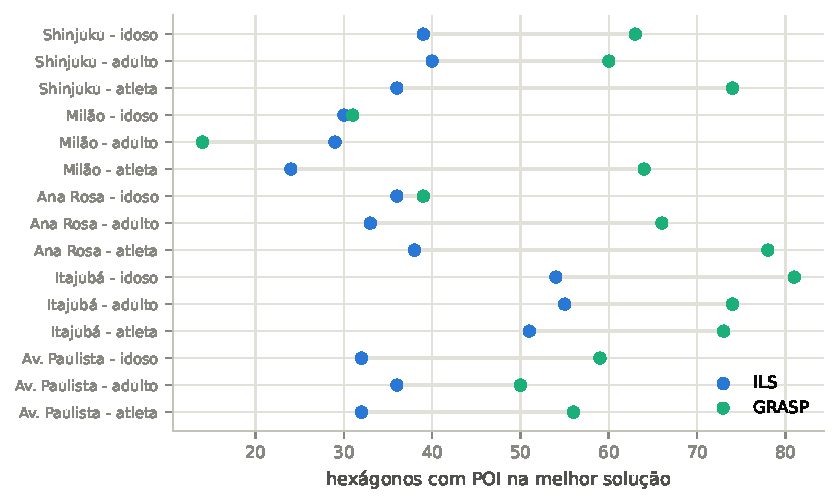
\includegraphics[width=0.8\textwidth]{figures/comp_alloc.pdf}
\caption{Número de hexágonos distintos que recebem POI na melhor solução de cada método, por instância.}
\label{fig:comp-alloc}
\end{figure}

\section{Efeito sobre a distribuição do IQC por hexágono}
\label{sec:comp-shape}

Os capítulos de cada método mostraram que ambos reduzem a assimetria positiva da distribuição do IQC entre hexágonos. A Tabela~\ref{tab:comp-shape} coloca os dois lado a lado. Das doze instâncias com assimetria inicial significativa, o método vencedor da instância produziu a menor assimetria final em onze — a exceção é Ana Rosa/atleta, em que o GRASP vence em valor mas o ILS termina com $g_1$ ligeiramente menor ($0{,}21$ contra $0{,}25$). Esse acoplamento entre vencer em soma e desconcentrar mais é coerente com o mecanismo comum aos dois métodos: sob a normalização min--max do IQC, elevar hexágonos da cauda baixa rende mais para a soma do que reforçar hexágonos já bons, então o método que atinge soma maior tende a ser o que mais achata a distribuição.

\renewcommand{\arraystretch}{1.12}
\begin{longtable}{@{}l l r r r r r r@{}}
\caption{Assimetria ($g_1$) e excesso de curtose ($g_2$) da distribuição do IQC por hexágono: antes da intervenção e após a melhor alocação de cada método. O símbolo $^{\dagger}$ marca valores significativamente diferentes de zero (D'Agostino, $5\%$).}\label{tab:comp-shape}\\
\toprule
Localidade & Perfil & $g_1$ antes & $g_1$ ILS & $g_1$ GRASP & $g_2$ antes & $g_2$ ILS & $g_2$ GRASP \\
\midrule
\endfirsthead
\toprule
Localidade & Perfil & $g_1$ antes & $g_1$ ILS & $g_1$ GRASP & $g_2$ antes & $g_2$ ILS & $g_2$ GRASP \\
\midrule
\endhead
av\_paulista & athlete & $+0{,}45^{\dagger}$ & $+0{,}29$ & $+0{,}06$ & $-0{,}37$ & $-0{,}35$ & $-0{,}89^{\dagger}$ \\
av\_paulista & average\_adult & $+0{,}52^{\dagger}$ & $+0{,}46^{\dagger}$ & $+0{,}10$ & $-0{,}24$ & $-0{,}01$ & $-1{,}06^{\dagger}$ \\
av\_paulista & elderly & $+0{,}58^{\dagger}$ & $+0{,}60^{\dagger}$ & $+0{,}28$ & $-0{,}07$ & $+0{,}17$ & $-0{,}60^{\dagger}$ \\
itajuba\_centro & athlete & $+0{,}82^{\dagger}$ & $+0{,}10$ & $+0{,}44^{\dagger}$ & $-0{,}34$ & $-0{,}99^{\dagger}$ & $-0{,}66^{\dagger}$ \\
itajuba\_centro & average\_adult & $+1{,}08^{\dagger}$ & $+0{,}05$ & $+0{,}50^{\dagger}$ & $+0{,}34$ & $-0{,}99^{\dagger}$ & $-0{,}35$ \\
itajuba\_centro & elderly & $+1{,}37^{\dagger}$ & $+0{,}54^{\dagger}$ & $+0{,}66^{\dagger}$ & $+1{,}48^{\dagger}$ & $-0{,}42$ & $-0{,}07$ \\
metro\_ana\_rosa & athlete & $+0{,}76^{\dagger}$ & $+0{,}21$ & $+0{,}25$ & $+0{,}33$ & $-0{,}79^{\dagger}$ & $-0{,}20$ \\
metro\_ana\_rosa & average\_adult & $+0{,}92^{\dagger}$ & $+0{,}47^{\dagger}$ & $+0{,}30$ & $+0{,}85$ & $-0{,}54$ & $-0{,}34$ \\
metro\_ana\_rosa & elderly & $+1{,}01^{\dagger}$ & $+0{,}86^{\dagger}$ & $+0{,}79^{\dagger}$ & $+1{,}03^{\dagger}$ & $+0{,}56$ & $+0{,}14$ \\
milao\_italia & athlete & $-0{,}09$ & $-0{,}11$ & $-0{,}15$ & $-0{,}93^{\dagger}$ & $-0{,}95^{\dagger}$ & $-0{,}92^{\dagger}$ \\
milao\_italia & average\_adult & $+0{,}01$ & $-0{,}03$ & $-0{,}13$ & $-0{,}84^{\dagger}$ & $-0{,}88^{\dagger}$ & $-0{,}99^{\dagger}$ \\
milao\_italia & elderly & $+0{,}13$ & $+0{,}09$ & $-0{,}00$ & $-0{,}62^{\dagger}$ & $-0{,}73^{\dagger}$ & $-0{,}82^{\dagger}$ \\
shinjuku\_toquio & athlete & $+0{,}63^{\dagger}$ & $+0{,}45^{\dagger}$ & $+0{,}44^{\dagger}$ & $-0{,}08$ & $-0{,}27$ & $-0{,}21$ \\
shinjuku\_toquio & average\_adult & $+0{,}77^{\dagger}$ & $+0{,}60^{\dagger}$ & $+0{,}49^{\dagger}$ & $+0{,}33$ & $+0{,}07$ & $-0{,}13$ \\
shinjuku\_toquio & elderly & $+0{,}88^{\dagger}$ & $+0{,}71^{\dagger}$ & $+0{,}56^{\dagger}$ & $+0{,}51$ & $+0{,}12$ & $-0{,}25$ \\
\bottomrule
\end{longtable}

\section{Síntese}
\label{sec:comp-sintese}

Os dados sustentam as seguintes conclusões, todas restritas às quinze instâncias, ao orçamento e às configurações testadas.

Primeiro, no nível por instância, as diferenças entre os métodos são grandes e inequívocas: todas as quinze comparações pareadas são significativas após Holm, com tamanhos de efeito $|r_{rb}| \ge 0{,}70$ e dominância completa por semente em nove instâncias. O GRASP obteve valores finais maiores em onze instâncias e o ILS em quatro (as três de Itajubá, por margens de $2{,}7$ a $6{,}3$ pontos de IQC, e Milão/atleta, por $0{,}31$).

Segundo, no nível agregado entre instâncias, a vantagem numérica do GRASP não é estatisticamente significativa (teste do sinal $p = 0{,}118$; Wilcoxon sobre as diferenças médias $p = 0{,}330$), porque as derrotas em Itajubá são muito maiores em módulo do que a maioria das vitórias. O resultado da comparação é, portanto, dependente da instância, e nenhum dos dois métodos domina o outro no conjunto testado.

Terceiro, os perfis de consumo de orçamento são opostos e explicam parte do quadro: o GRASP converge cedo e para por estagnação em $100\%$ das execuções, com cerca de um terço do teto de avaliações; o ILS usa o teto em $97{,}4\%$ das execuções e continua melhorando até o fim. Sob orçamento igual, o placar por instância é o mesmo a partir de $5\,000$ avaliações, mas a vantagem do ILS em Itajubá cresce com o orçamento, e Milão/atleta muda de mãos ao longo dele. Na métrica de avaliações até o alvo, o GRASP alcança a média final do ILS com menos de $600$ avaliações (mediana) em oito das onze instâncias que vence; o ILS alcança a média final do GRASP com medianas de $648$ a $1\,461$ avaliações nas três que vence.

Quarto, os métodos produzem soluções estruturalmente distintas: as melhores alocações do GRASP espalham os POIs por mais hexágonos ($58{,}8$ contra $37{,}7$ em média) e com menor concentração (HHI $0{,}033$ contra $0{,}058$), e a sobreposição espacial entre as soluções dos dois métodos é baixa (Jaccard médio $0{,}24$). A dispersão entre sementes difere significativamente em oito instâncias, sem direção uniforme, e a correlação semente a semente entre os métodos é desprezível.

Quinto, os dois métodos reduzem a assimetria da distribuição do IQC entre hexágonos, e o método que vence em soma é também, em onze das doze instâncias inicialmente assimétricas, o que mais reduz a assimetria — consequência da normalização min--max, sob a qual elevar a cauda baixa é o caminho mais rentável para a soma.

\end{document}
